\section{Muon momentum calibration}
\label{muon_calib}

With a theoretical width of around 5 MeV, the Higgs peak is dominated by the detector resolution which is on the order of a GeV. With such a narrow theoretical width, improving the dimuon mass resolution in data is an important factor in the sensitivity of the analysis. Moreover, the the mean and the resolution of the dimuon mass peaks in Monte Carlo, namely the Higgs peak, must match in data in order to set limits accurately. CMSSW provides two packages to address these issues, the Rochester Muon Corrections and the Kalman Filter Muon Corrections. In the following studies the Z peak is fit with a Voigtian and the fit mean and experimental resolution are extracted and plotted against various muon kinematics.

\subsection{Muon Corrections in Data}

In this section, the muon corrections are studied in data. Figure \ref{fig:net_data_mu_calib_mean} shows the mean of the Z peak plotted vs phi plus, phi minus, eta plus, eta minus, pt plus, pt minus, and the dimuon pt for the Rochester, Kalman Filter, and uncorrected Particle Flow predictions. Here plus and minus refer to the positive or negative muon in the dimuon event respectively. After corrections, the mean is shifted closer to the theoretical value of 91.2 GeV. Furthermore, the Rochester corrections reduce the variation in phi from 0.1 GeV to 0.0025 GeV an improvement of 98\%.

\begin{figure}[hbp]
  \centering
  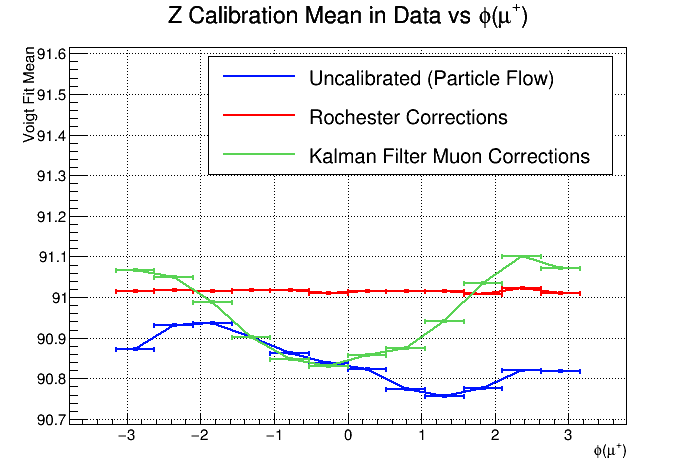
\includegraphics[width=0.32\linewidth]{figures/muon_calib/zcal_data_mean_phi_plus.png}
  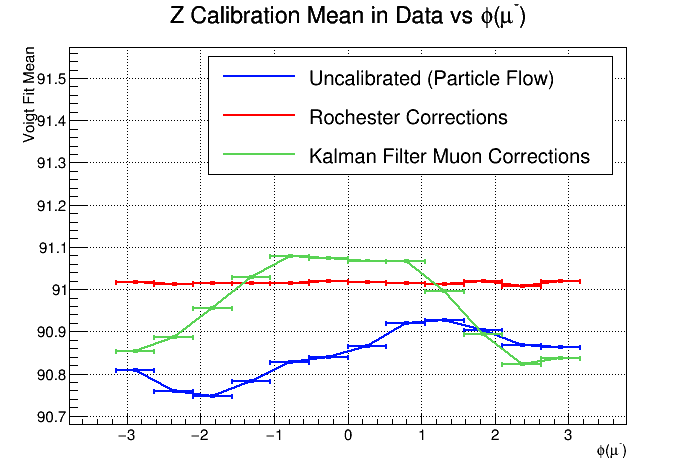
\includegraphics[width=0.32\linewidth]{figures/muon_calib/zcal_data_mean_phi_minus.png}
  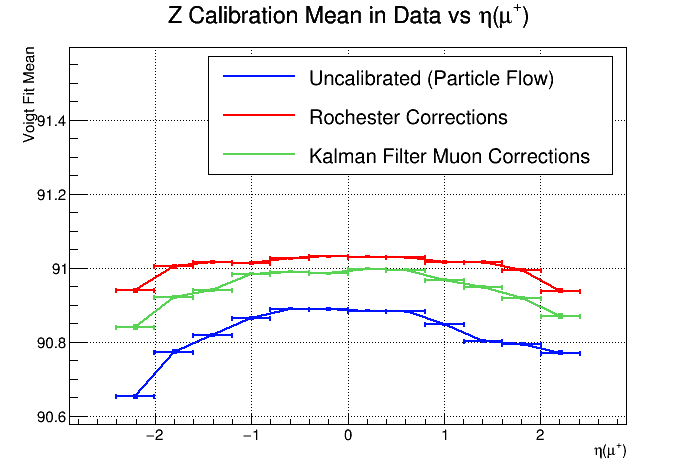
\includegraphics[width=0.32\linewidth]{figures/muon_calib/zcal_data_mean_eta_plus.png}
  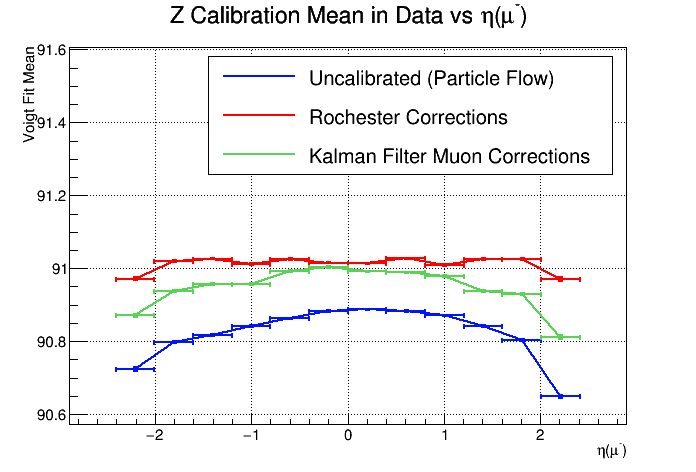
\includegraphics[width=0.32\linewidth]{figures/muon_calib/zcal_data_mean_eta_minus.png}
  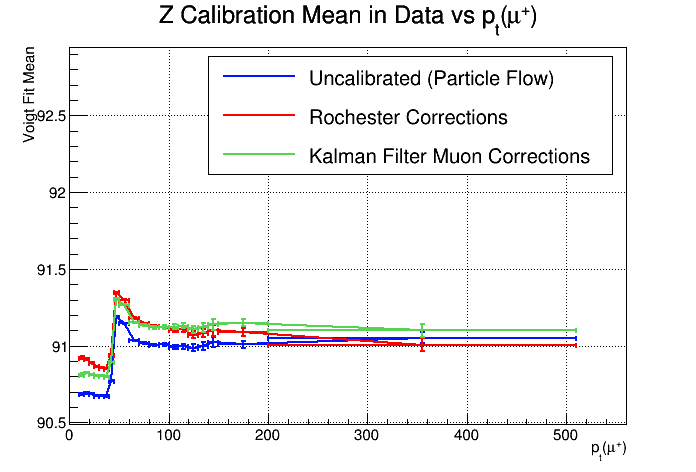
\includegraphics[width=0.32\linewidth]{figures/muon_calib/zcal_data_mean_pt_plus.png}
  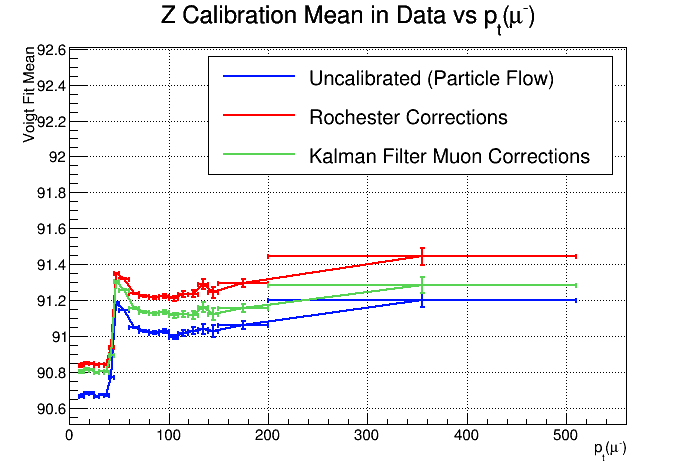
\includegraphics[width=0.32\linewidth]{figures/muon_calib/zcal_data_mean_pt_minus.png}
  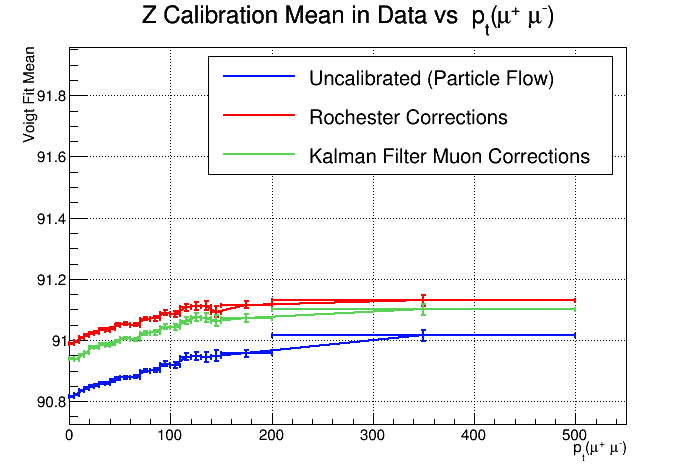
\includegraphics[width=0.32\linewidth]{figures/muon_calib/zcal_data_mean_dimu_pt.png}
  \caption
   {The Rochester (Roch) and Kalman Filter (KaMu) muon corrections applied to data and compared to the uncalibrated Particle Flow (PF) mass in terms of the mean.}
  \label{fig:net_data_mu_calib_mean}
\end{figure}

Figure \ref{fig:net_data_mu_calib_res} shows the Z resolution plotted against the same variables. The Rochester corrections improve the Z resolution by 1.6\%, which translates to about 20 MeV, roughly 4 theoretical Higgs widths. The Kalman filter corrections improve the resolution in data by 0.076\% about 10 MeV or 2 theoretical Higgs widths.

\begin{figure}[hbp]
  \centering
  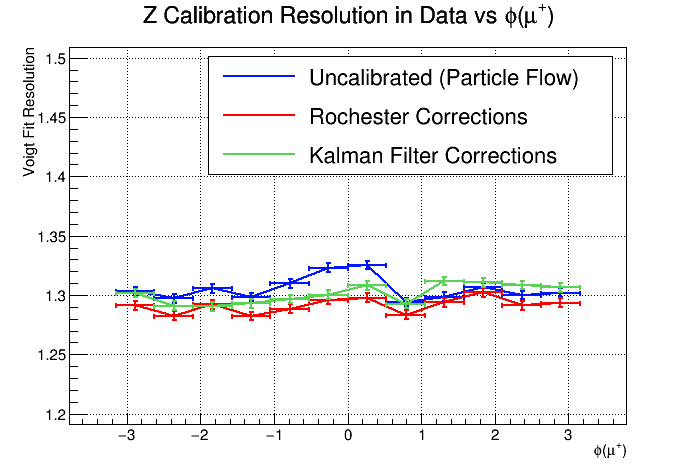
\includegraphics[width=0.32\linewidth]{figures/muon_calib/zcal_data_res_phi_plus.png}
  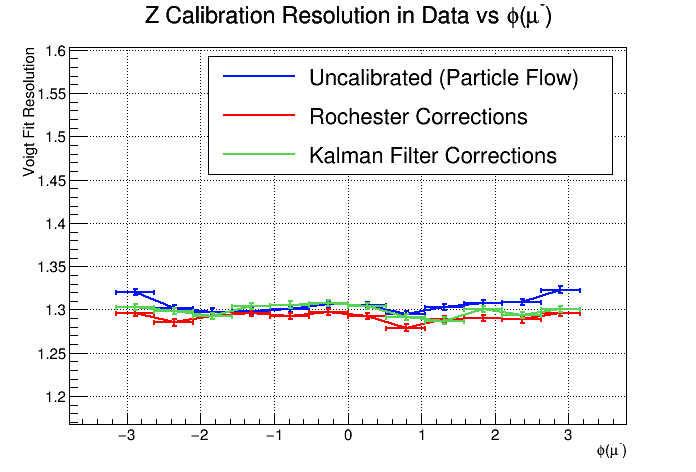
\includegraphics[width=0.32\linewidth]{figures/muon_calib/zcal_data_res_phi_minus.png}
  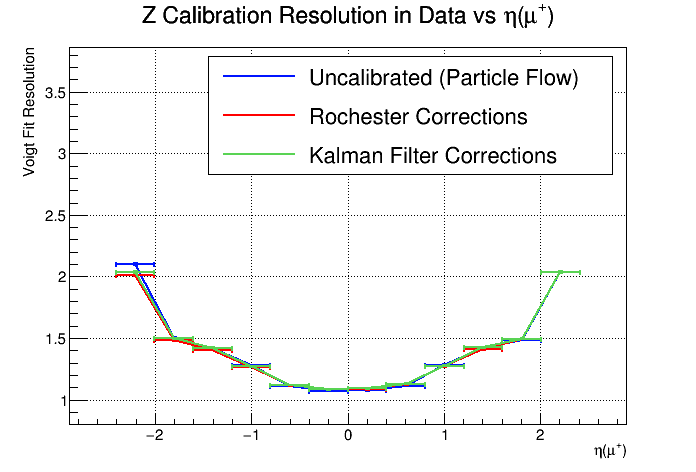
\includegraphics[width=0.32\linewidth]{figures/muon_calib/zcal_data_res_eta_plus.png}
  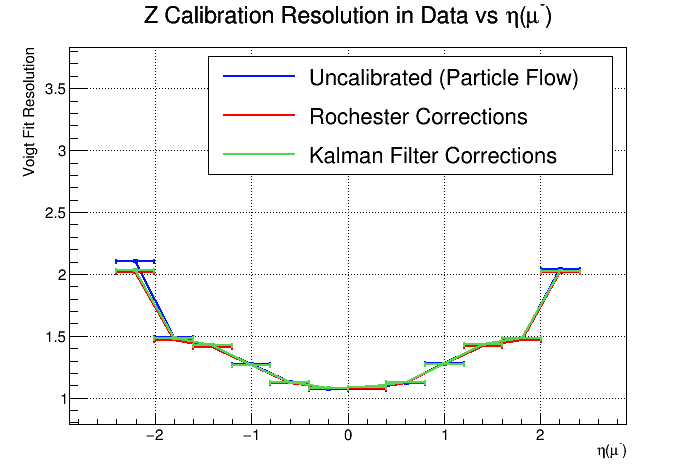
\includegraphics[width=0.32\linewidth]{figures/muon_calib/zcal_data_res_eta_minus.png}
  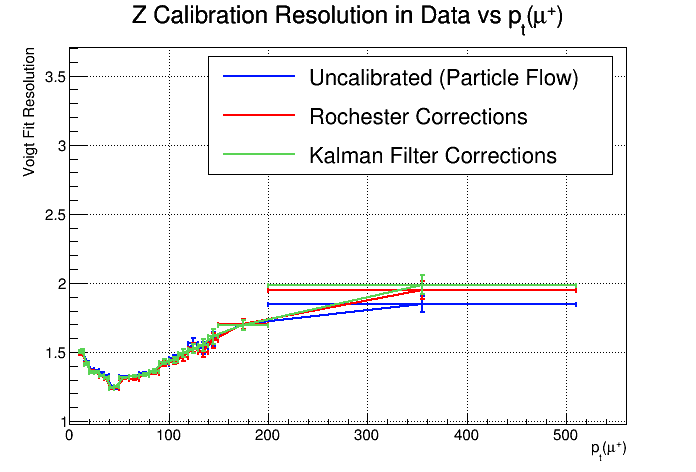
\includegraphics[width=0.32\linewidth]{figures/muon_calib/zcal_data_res_pt_plus.png}
  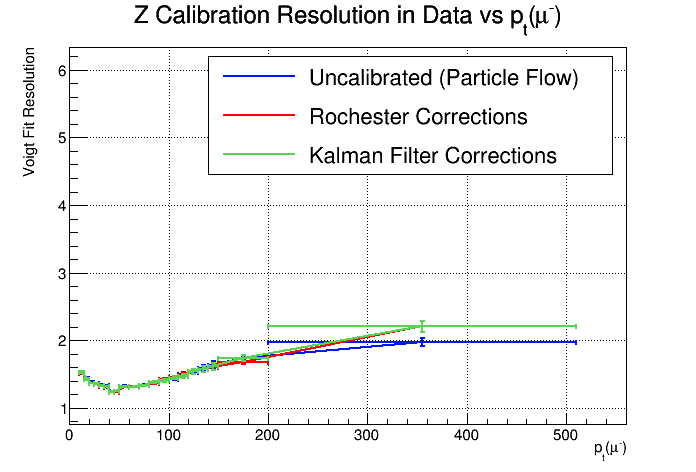
\includegraphics[width=0.32\linewidth]{figures/muon_calib/zcal_data_res_pt_minus.png}
  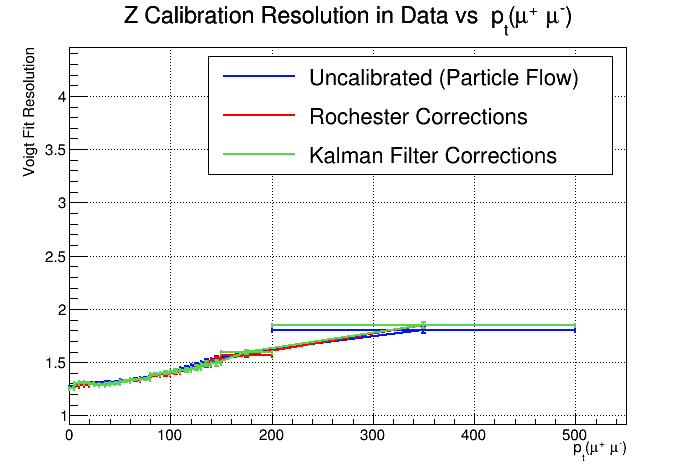
\includegraphics[width=0.32\linewidth]{figures/muon_calib/zcal_data_res_dimu_pt.png}
  \caption
   {The Rochester (Roch) and Kalman Filter (KaMu) muon corrections applied to data and compared to the uncalibrated Particle Flow (PF) mass in terms of resolution.}
  \label{fig:net_data_mu_calib_res}
\end{figure}

\subsection{Data-MC agreement in scale, resolution}

As aforementioned the muon corrections should not only improve the resolution of the dimuon mass peaks in data, but align the scale and resolution between data and Monte Carlo as well. Figure \ref{fig:data_mc_mean_before} shows the Data/MC agreement on the Z peak mean before any corrections, while figure \ref{fig:data_mc_roch_mean_after} shows the agreement after Rochester corrections and \ref{fig:data_mc_kamu_mean_after} shows the agreement after the Kalman filter muon corrections. Both the Rochester and Kalman muon corrections successfully align Data/MC in terms of the Z peak mean.

\begin{figure}[hbp]
  \centering
  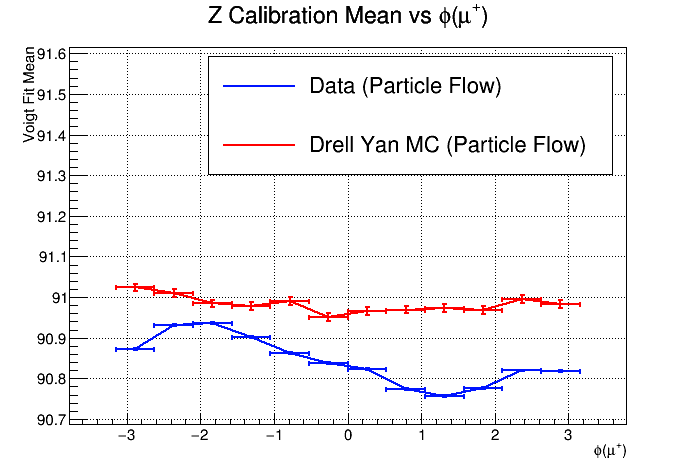
\includegraphics[width=0.32\linewidth]{figures/muon_calib/zcal_pf_mc-data_mean_phi_plus.png}
  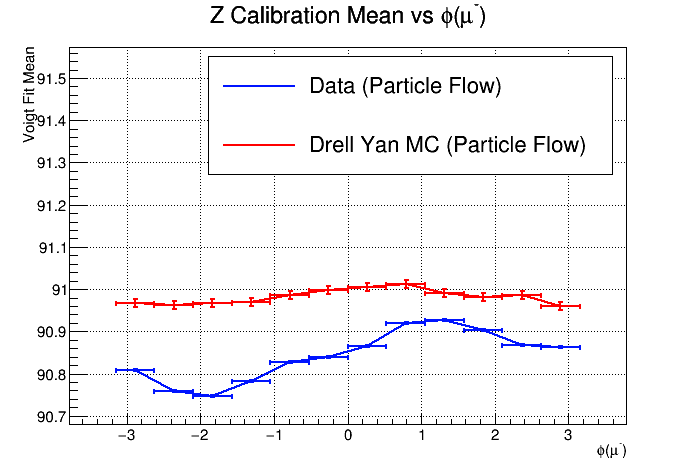
\includegraphics[width=0.32\linewidth]{figures/muon_calib/zcal_pf_mc-data_mean_phi_minus.png}
  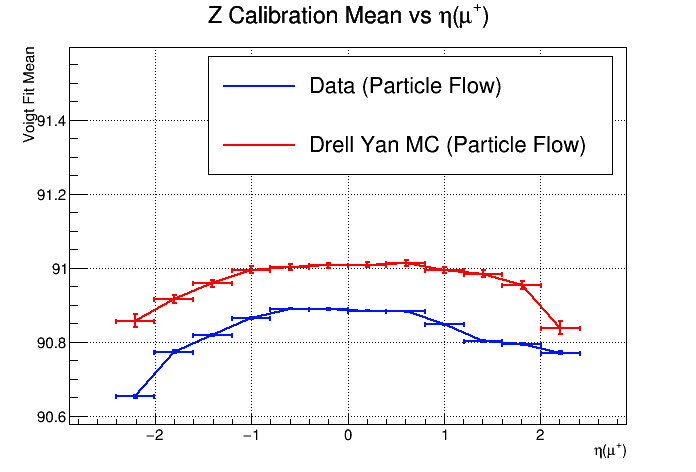
\includegraphics[width=0.32\linewidth]{figures/muon_calib/zcal_pf_mc-data_mean_eta_plus.png}
  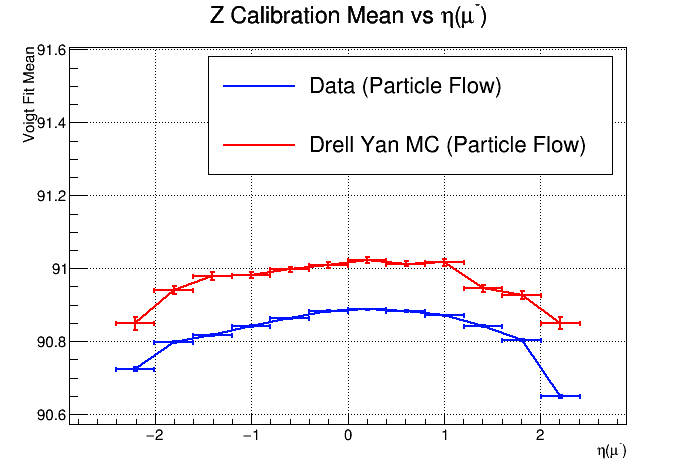
\includegraphics[width=0.32\linewidth]{figures/muon_calib/zcal_pf_mc-data_mean_eta_minus.png}
  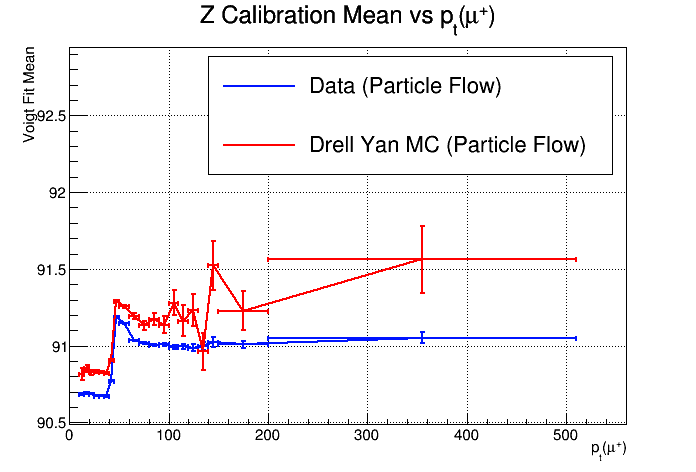
\includegraphics[width=0.32\linewidth]{figures/muon_calib/zcal_pf_mc-data_mean_pt_plus.png}
  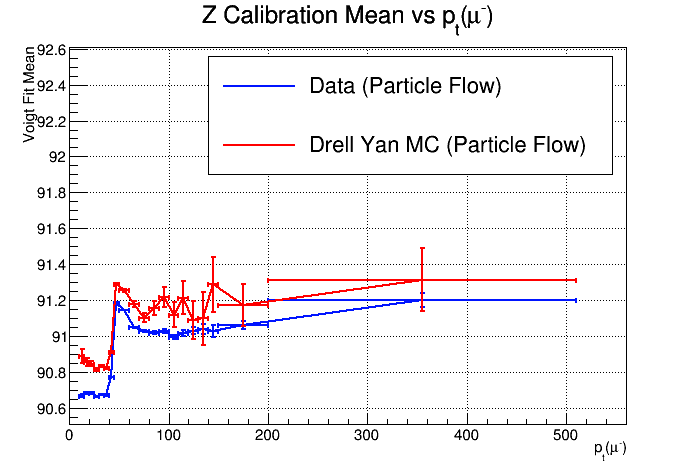
\includegraphics[width=0.32\linewidth]{figures/muon_calib/zcal_pf_mc-data_mean_pt_minus.png}
  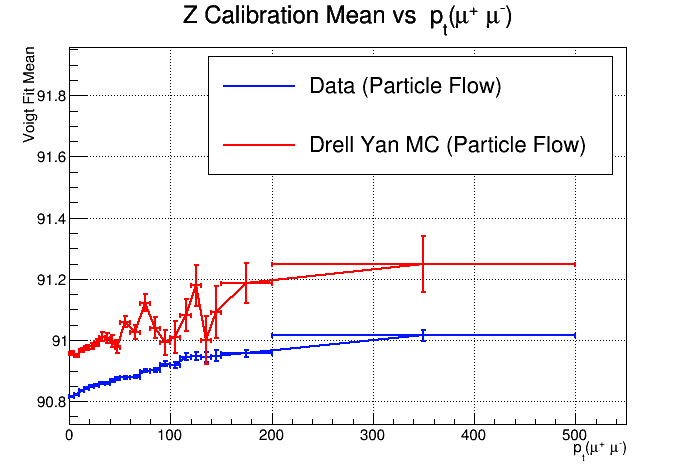
\includegraphics[width=0.32\linewidth]{figures/muon_calib/zcal_pf_mc-data_mean_dimu_pt.png}
  \caption
   {Data and MC are not in alignment in terms of the Z peak mean before corrections.}
  \label{fig:data_mc_mean_before}
\end{figure}

\begin{figure}[hbp]
  \centering
  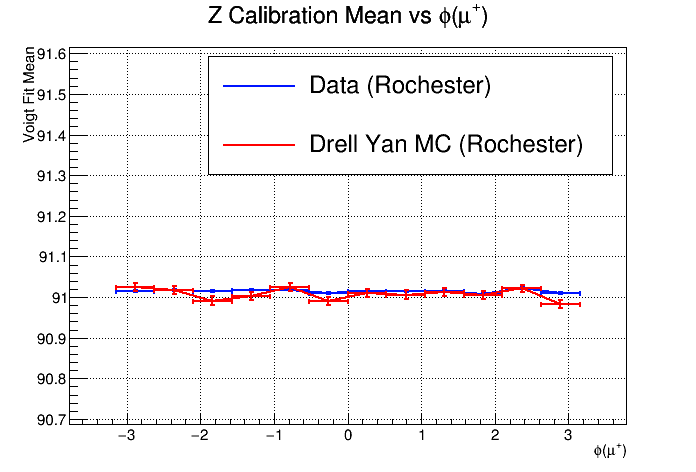
\includegraphics[width=0.32\linewidth]{figures/muon_calib/zcal_roch_mc-data_mean_phi_plus.png}
  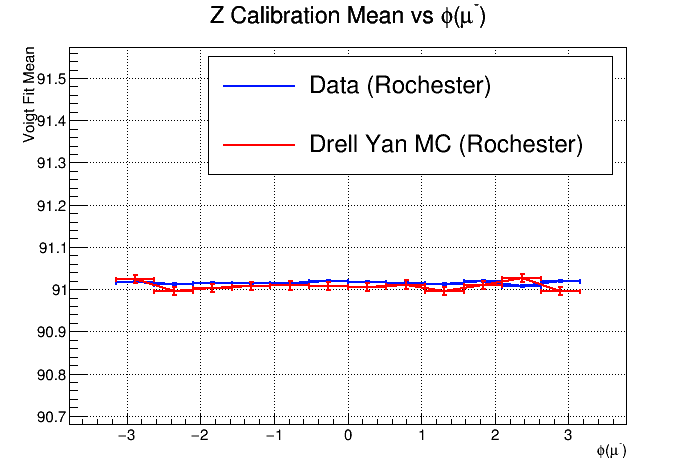
\includegraphics[width=0.32\linewidth]{figures/muon_calib/zcal_roch_mc-data_mean_phi_minus.png}
  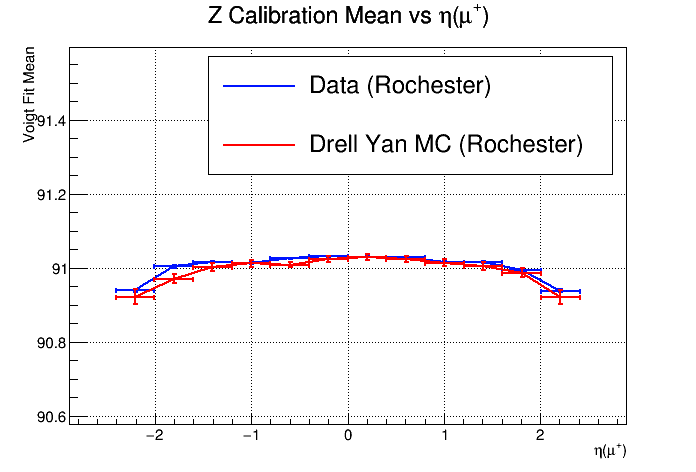
\includegraphics[width=0.32\linewidth]{figures/muon_calib/zcal_roch_mc-data_mean_eta_plus.png}
  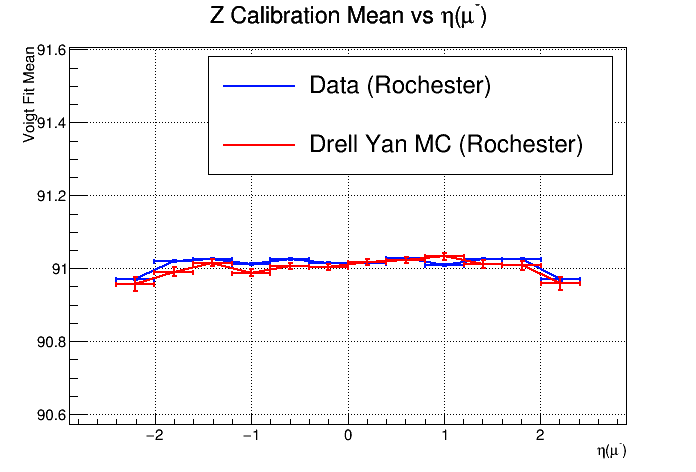
\includegraphics[width=0.32\linewidth]{figures/muon_calib/zcal_roch_mc-data_mean_eta_minus.png}
  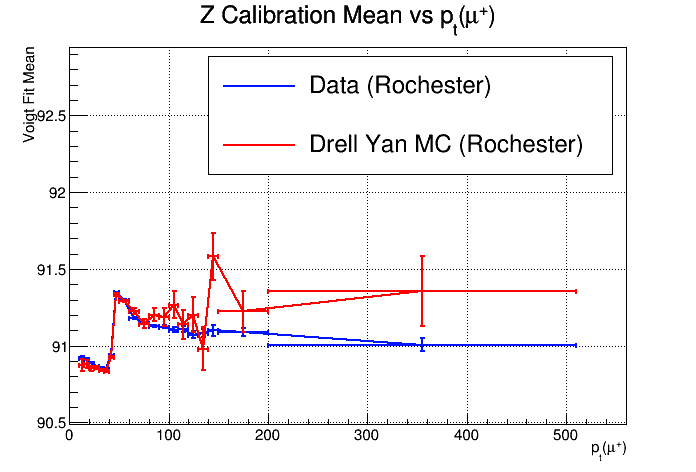
\includegraphics[width=0.32\linewidth]{figures/muon_calib/zcal_roch_mc-data_mean_pt_plus.png}
  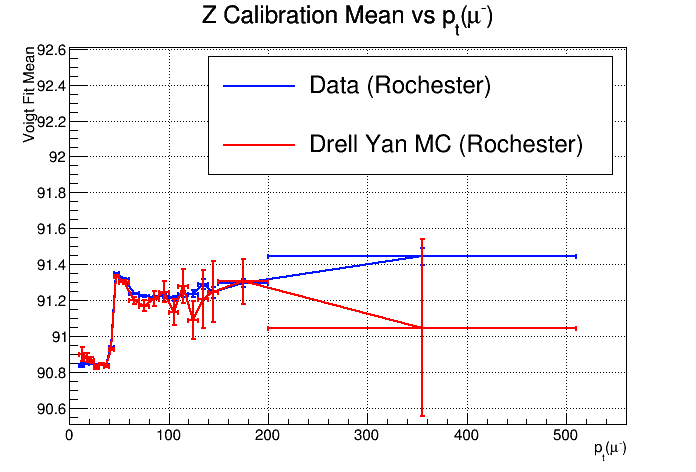
\includegraphics[width=0.32\linewidth]{figures/muon_calib/zcal_roch_mc-data_mean_pt_minus.png}
  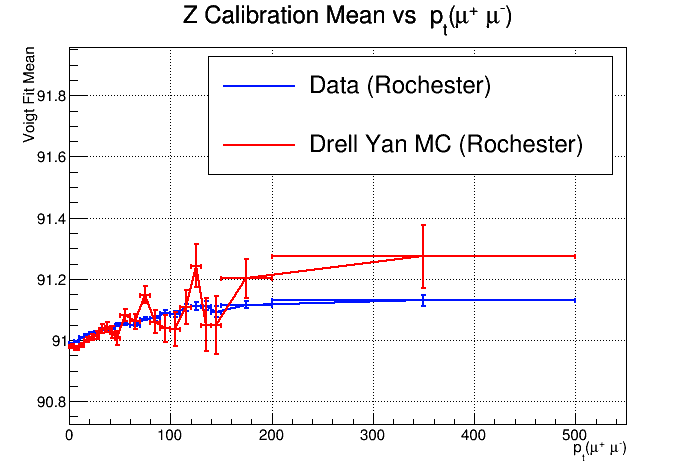
\includegraphics[width=0.32\linewidth]{figures/muon_calib/zcal_roch_mc-data_mean_dimu_pt.png}
  \caption
   {Data and MC align very well in terms of the Z peak mean after applying the Rochester muon corrections.}
  \label{fig:data_mc_roch_mean_after}
\end{figure}

\begin{figure}[hbp]
  \centering
  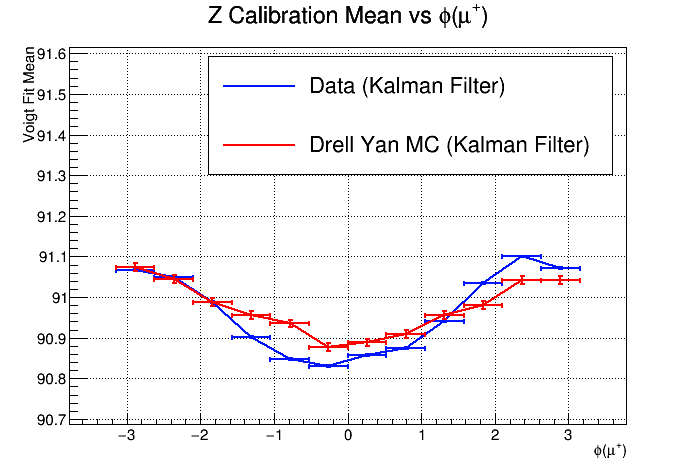
\includegraphics[width=0.32\linewidth]{figures/muon_calib/zcal_kamu_mc-data_mean_phi_plus.png}
  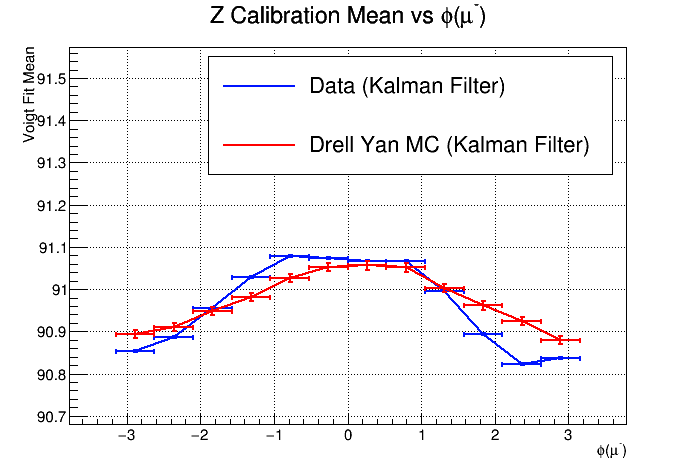
\includegraphics[width=0.32\linewidth]{figures/muon_calib/zcal_kamu_mc-data_mean_phi_minus.png}
  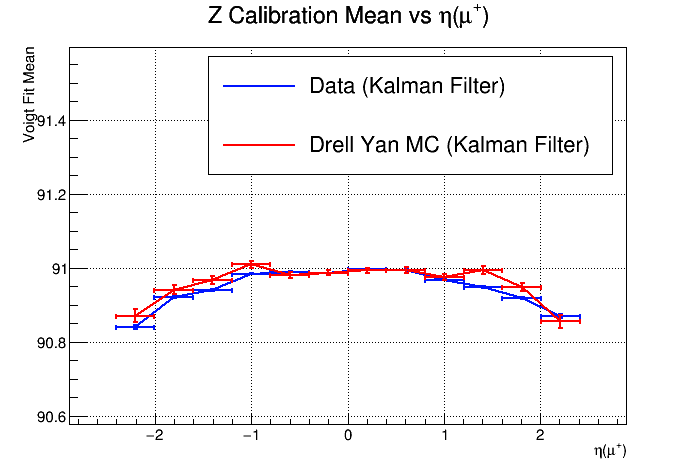
\includegraphics[width=0.32\linewidth]{figures/muon_calib/zcal_kamu_mc-data_mean_eta_plus.png}
  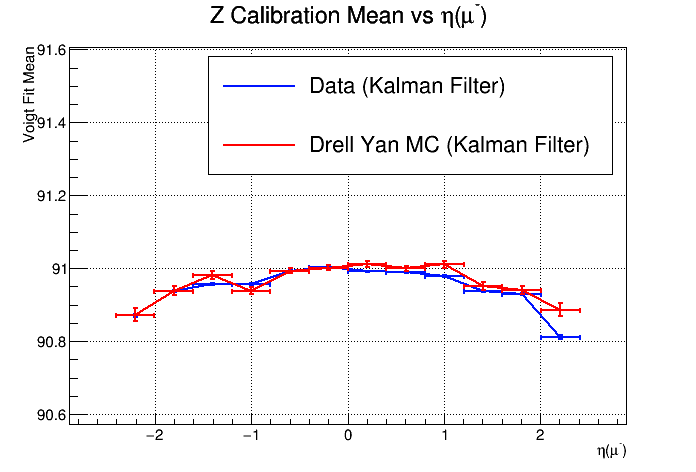
\includegraphics[width=0.32\linewidth]{figures/muon_calib/zcal_kamu_mc-data_mean_eta_minus.png}
  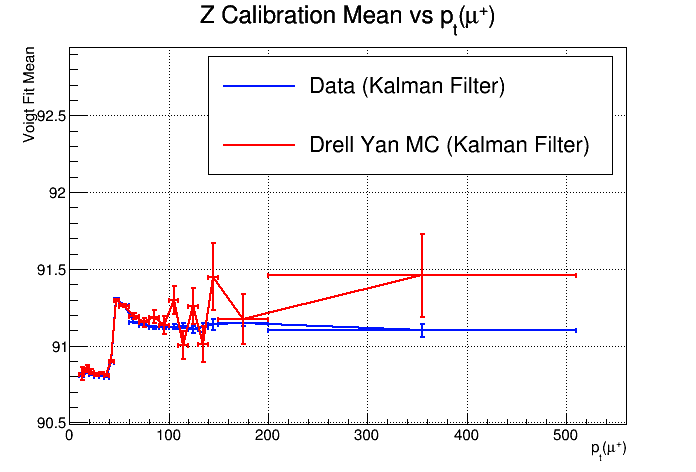
\includegraphics[width=0.32\linewidth]{figures/muon_calib/zcal_kamu_mc-data_mean_pt_plus.png}
  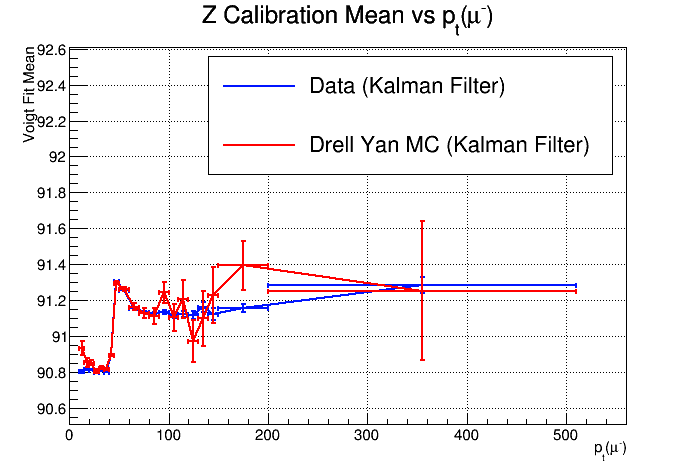
\includegraphics[width=0.32\linewidth]{figures/muon_calib/zcal_kamu_mc-data_mean_pt_minus.png}
  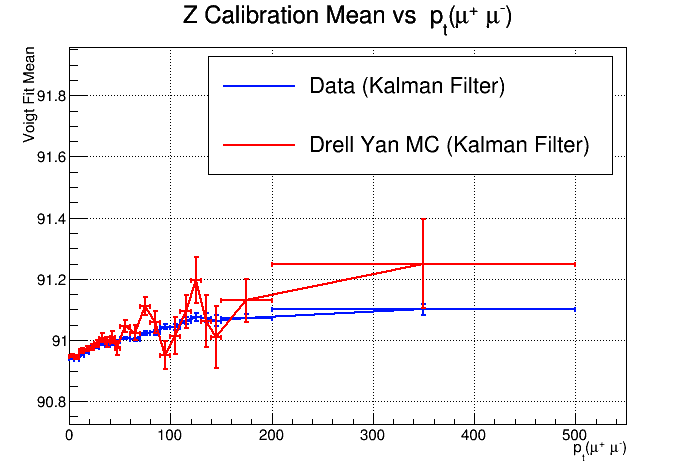
\includegraphics[width=0.32\linewidth]{figures/muon_calib/zcal_kamu_mc-data_mean_dimu_pt.png}
  \caption
   {Data and MC align very well in terms of the Z peak mean after applying the Kalman filter muon corrections.}
  \label{fig:data_mc_kamu_mean_after}
\end{figure}

Both corrections also succeed in aligning the Z peak resolution. The mismatch before corrections is seen in Figure \ref{fig:data_mc_res_before} and the agreement after corrections is seen in Figure \ref{fig:data_mc_roch_res_after} and Figure \ref{fig:data_mc_kamu_res_after}.

\begin{figure}[hbp]
  \centering
  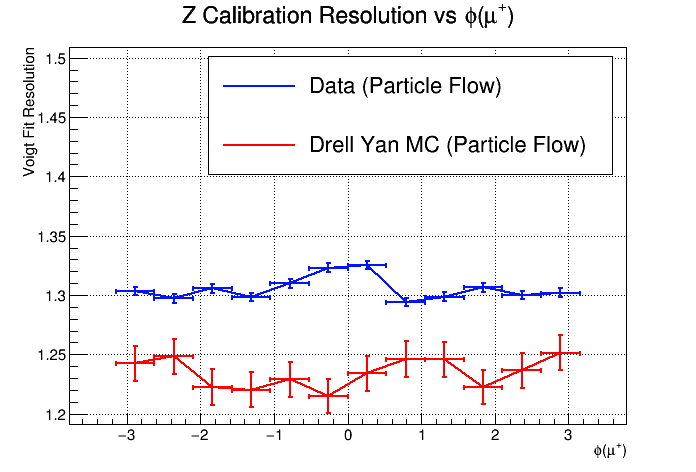
\includegraphics[width=0.32\linewidth]{figures/muon_calib/zcal_pf_mc-data_res_phi_plus.png}
  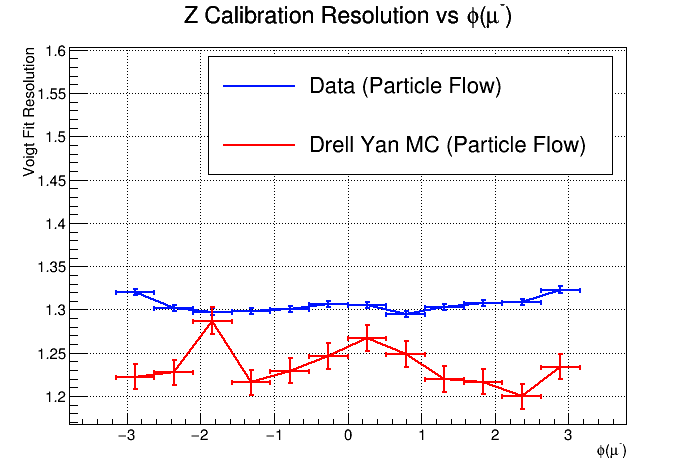
\includegraphics[width=0.32\linewidth]{figures/muon_calib/zcal_pf_mc-data_res_phi_minus.png}
  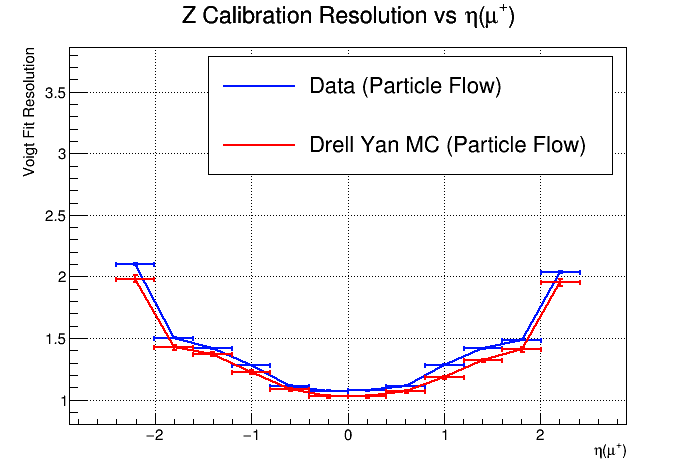
\includegraphics[width=0.32\linewidth]{figures/muon_calib/zcal_pf_mc-data_res_eta_plus.png}
  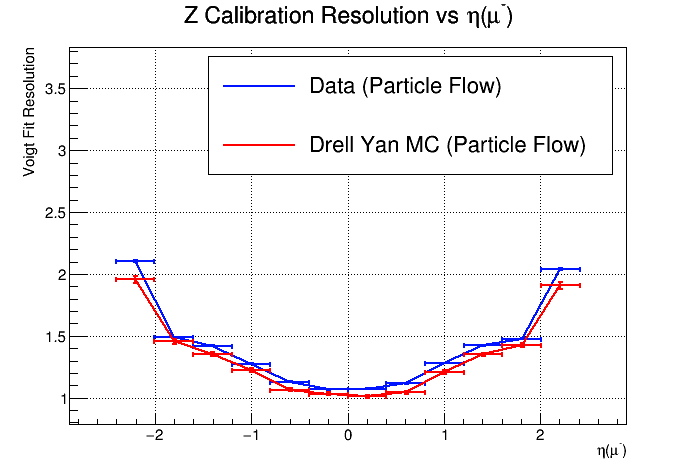
\includegraphics[width=0.32\linewidth]{figures/muon_calib/zcal_pf_mc-data_res_eta_minus.png}
  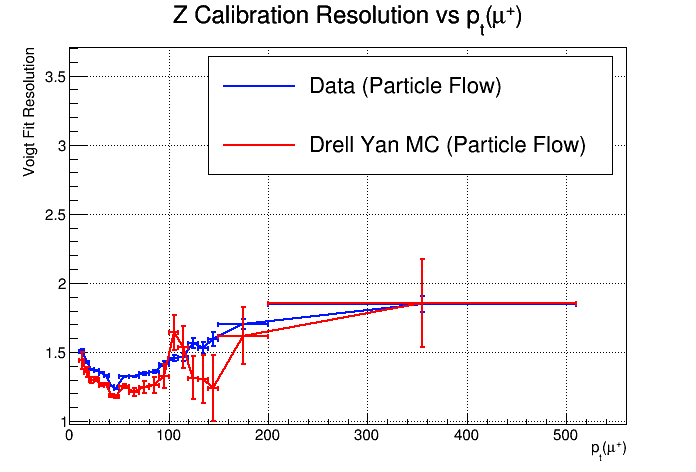
\includegraphics[width=0.32\linewidth]{figures/muon_calib/zcal_pf_mc-data_res_pt_plus.png}
  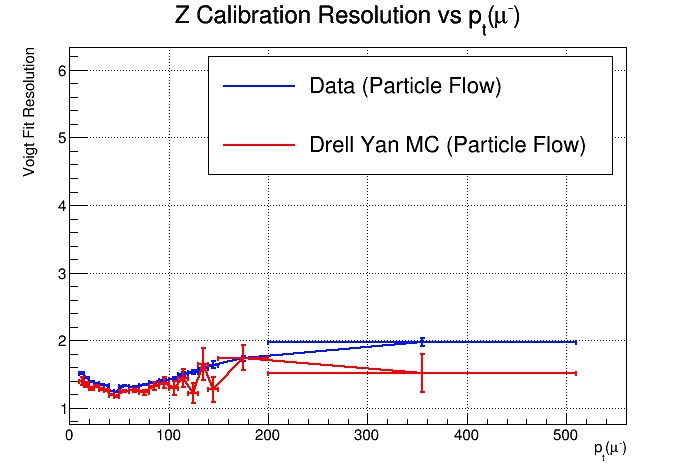
\includegraphics[width=0.32\linewidth]{figures/muon_calib/zcal_pf_mc-data_res_pt_minus.png}
  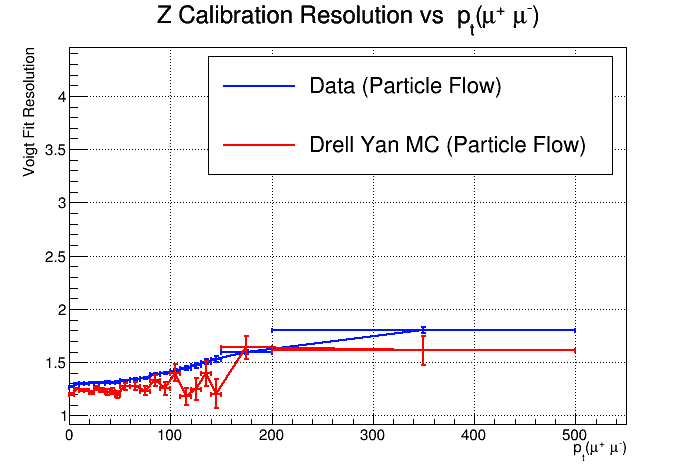
\includegraphics[width=0.32\linewidth]{figures/muon_calib/zcal_pf_mc-data_res_dimu_pt.png}
  \caption
   {Data and MC do not show similar resolutions for the Z peak before corrections.}
  \label{fig:data_mc_res_before}
\end{figure}

\begin{figure}[hbp]
  \centering
  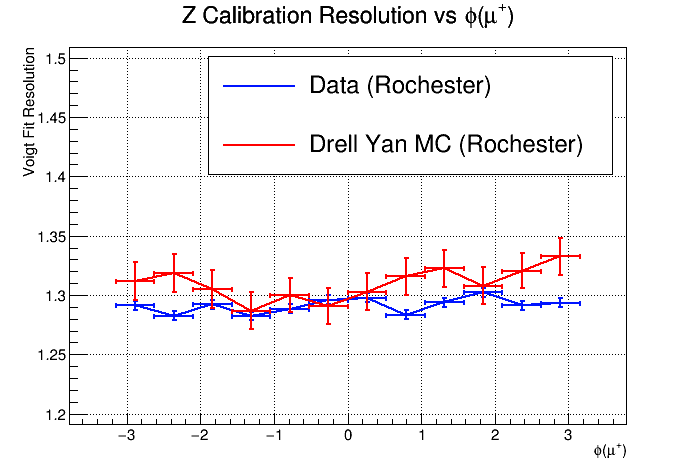
\includegraphics[width=0.32\linewidth]{figures/muon_calib/zcal_roch_mc-data_res_phi_plus.png}
  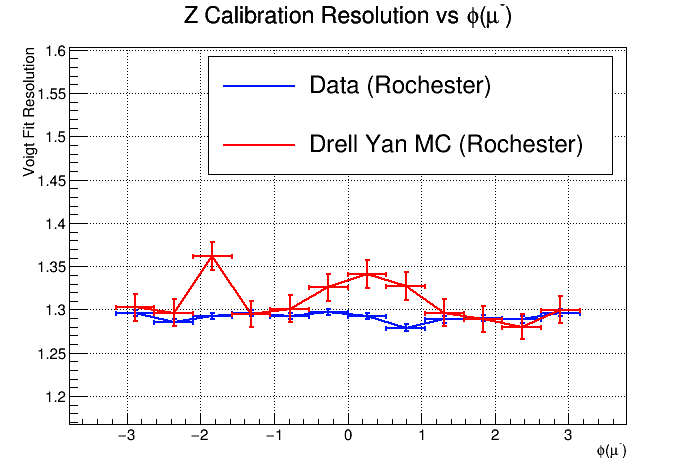
\includegraphics[width=0.32\linewidth]{figures/muon_calib/zcal_roch_mc-data_res_phi_minus.png}
  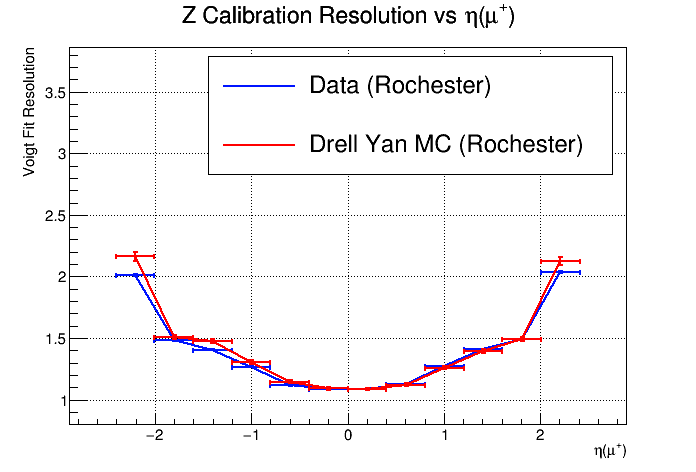
\includegraphics[width=0.32\linewidth]{figures/muon_calib/zcal_roch_mc-data_res_eta_plus.png}
  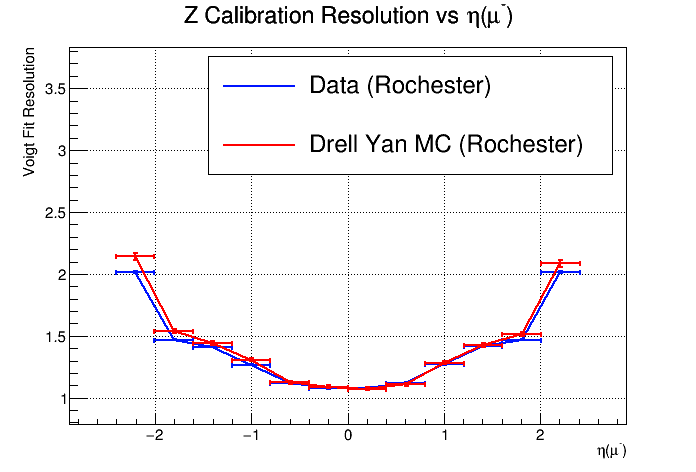
\includegraphics[width=0.32\linewidth]{figures/muon_calib/zcal_roch_mc-data_res_eta_minus.png}
  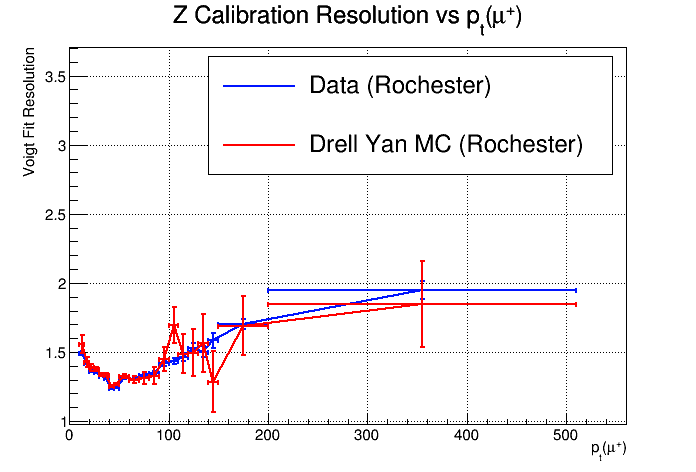
\includegraphics[width=0.32\linewidth]{figures/muon_calib/zcal_roch_mc-data_res_pt_plus.png}
  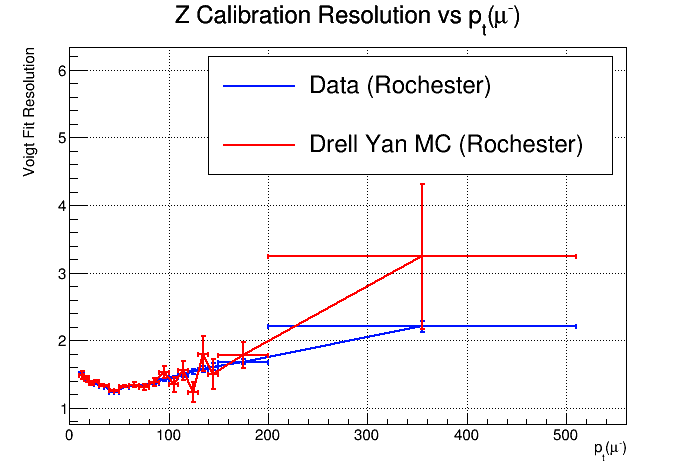
\includegraphics[width=0.32\linewidth]{figures/muon_calib/zcal_roch_mc-data_res_pt_minus.png}
  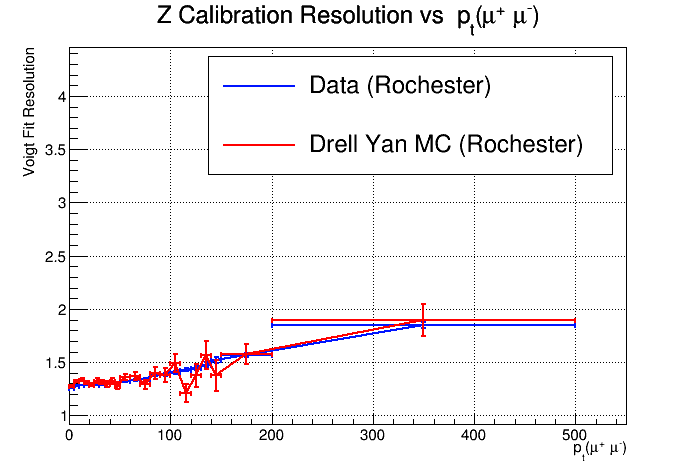
\includegraphics[width=0.32\linewidth]{figures/muon_calib/zcal_roch_mc-data_res_dimu_pt.png}
  \caption
   {After Rochester corrections data and MC have similar resolutions for the Z peak.}
  \label{fig:data_mc_roch_res_after}
\end{figure}

\begin{figure}[hbp]
  \centering
  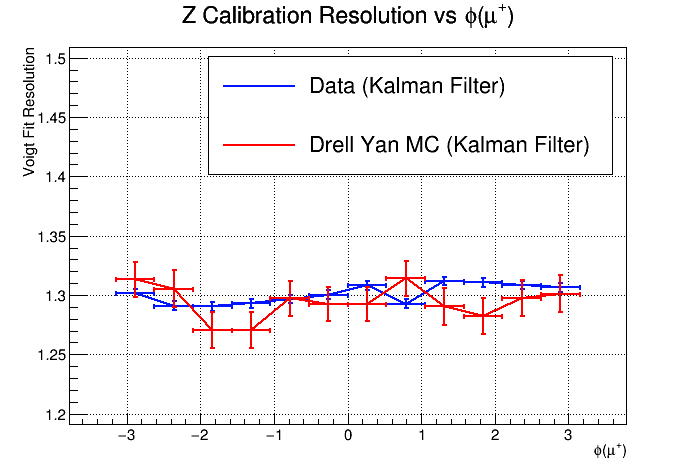
\includegraphics[width=0.32\linewidth]{figures/muon_calib/zcal_kamu_mc-data_res_phi_plus.png}
  \includegraphics[width=0.32\linewidth]{figures/muon_calib/zcal_kamu_mc-data_res_phi_minus.png}
  \includegraphics[width=0.32\linewidth]{figures/muon_calib/zcal_kamu_mc-data_res_eta_plus.png}
  \includegraphics[width=0.32\linewidth]{figures/muon_calib/zcal_kamu_mc-data_res_eta_minus.png}
  \includegraphics[width=0.32\linewidth]{figures/muon_calib/zcal_kamu_mc-data_res_pt_plus.png}
  \includegraphics[width=0.32\linewidth]{figures/muon_calib/zcal_kamu_mc-data_res_pt_minus.png}
  \includegraphics[width=0.32\linewidth]{figures/muon_calib/zcal_kamu_mc-data_res_dimu_pt.png}
  \caption
   {After Rochester corrections data and MC have similar resolutions for the Z peak.}
  \label{fig:data_mc_kamu_res_after}
\end{figure}
\subsection{Derivation of systematic uncertainties}
